% Created 2019-12-05 Thu 23:24
% Intended LaTeX compiler: pdflatex
\documentclass[11pt]{article}
\usepackage[utf8]{inputenc}
\usepackage[T1]{fontenc}
\usepackage{graphicx}
\usepackage{grffile}
\usepackage{longtable}
\usepackage{wrapfig}
\usepackage{rotating}
\usepackage[normalem]{ulem}
\usepackage{amsmath}
\usepackage{textcomp}
\usepackage{amssymb}
\usepackage{capt-of}
\usepackage{hyperref}
\setlength{\parindent}{0pt}
\author{Louis James}
\date{\today}
\title{Project Specification - Cognitive aspects of HCI in \emph{"the dynamic medium"}}
\hypersetup{
 pdfauthor={Louis James},
 pdftitle={Project Specification - Cognitive aspects of HCI in \emph{"the dynamic medium"}},
 pdfkeywords={},
 pdfsubject={},
 pdfcreator={Emacs 26.3 (Org mode 9.2.6)}, 
 pdflang={English}}
\begin{document}

\maketitle
\section*{Project overview}
\label{sec:org6a5c688}

In this project I will create a browser based system for spatial tabletop computer interaction. It will be web based interactive \{computing\} environment where one can \emph{write programs} by arranging coloured objects on the table. When put in particular patterns this will trigger an affect. This could be displaying an image or connecting objects in the space, displaying a text editor or a web page. The fundamental idea here would be an interaction model based of physical placement and movement of objects on a 2d surface space which then reacts live.\\

\begin{figure}[htbp]
\centering
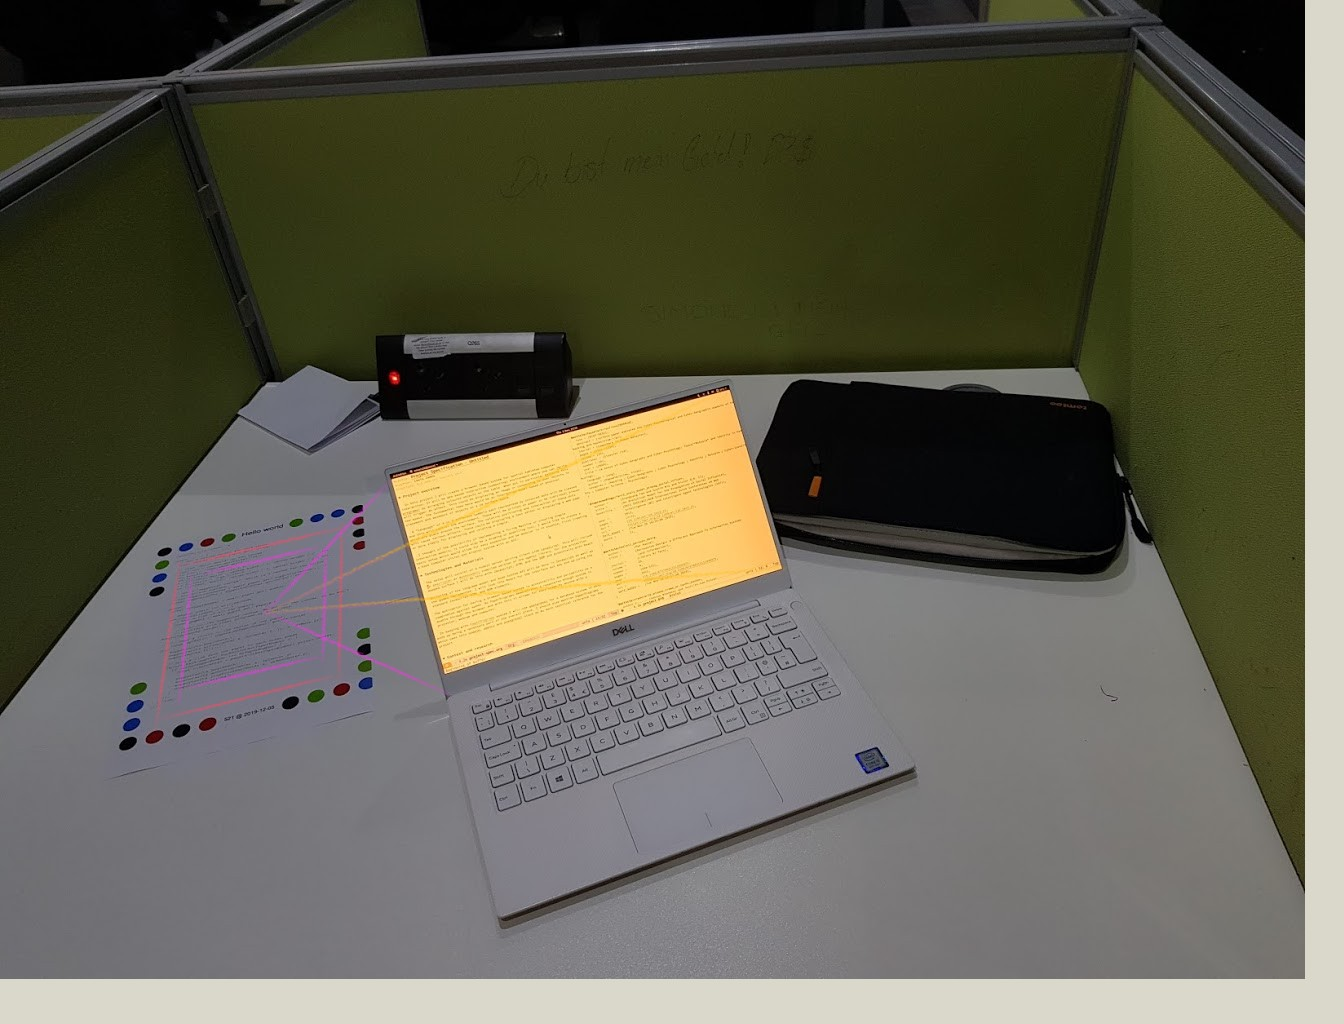
\includegraphics[width=.9\linewidth]{setup.jpg}
\caption{sketch 1}
\end{figure}

A set of 4 or 5 different symbols each represented by coloured dots will be created and this will control the environment. These will be printed on paper or be individual pieces which are place around the surface. The relative positioning and interaction of these dots will cause various effects.\\

I thought of the possibility of implementing a Turing Machine but the first thing would be creating simple interactive models; this could also be a drawing or modelling tool or game. I would like to create a base setup which would allow for easy expansion and be modular in it's essence, first creating a base Computer vision and display system with an API following this an interaction design style game experiment. This could be something relatively simple but it would be a game that facilitates an exploration of the cognitive aspects of \emph{human computer interaction}.\\

\section*{Technologies and Materials}
\label{sec:orgc19dab9}

The setup will consist of a nodejs server serving client side javascript. This will include an \href{https://docs.opencv.org/3.4/d4/da1/tutorial\_js\_setup.html}{emscripten} or \href{https://webassembly.org/}{WebAssembly} compiled version of the opencv library. For the projection mapped surface I will do this with Javascript, HTML and the DOM and potentially with \href{https://reactjs.org/}{React Js}. Scripting of the language model and base system API will be done in Javascript as well as the games implemented. I will look into React for the interface but may end up using the standard Javascript, HTML and DOM elements.\\

The motivation for having a browser based system is accessibility and portability as a compromise over speed. As PaperPrograms demonstrates a responsive enough system is doable through the browser and with this it allows for easy usage by anyone with a projector, webcam and computer. In keeping with \href{https://paperprograms.org/}{PaperProgram's} system I will use postgresql for a database system if this ends up being a necessary part of the overall piece. I should also formally mention PaperPrograms, which uses this nodejs, opencv and postgresql stack, as my main technical reference for the project.\\

Hardware will consist of my laptop running locally the node server and client system as well as a projector; PaperPrograms recommend 1080p and at least 2000 Limns. Colour printing and potentially colour pens or some other source of coloured paper. Colour printing should be good for consistent colour.\\

\section*{Context and research}
\label{sec:org00d76ea}

My main point of reference is \href{https://dynamicland.org}{Dynamicland} \cite{VictorKayDynamicLand}, an immersive collaborative computer system based in Oakland (US), and more specifically PaperPrograms, a web implementation of one element of Dynamicland's \emph{Realtalk OS}. \emph{PaperPrograms} is a camera, projector and computer setup where colour pattern coded  pieces of paper are recognised by a camera and corresponding Javascript programs are then run and the results of which are projected onto the same surface. This creates a loop where program-object has physical representation on a surface; it's position and relation to other programs can have effects on the overall system.\\

Through the project I would like to explore the cognitive aspects of \emph{Human Computer Interaction} \cite{SharpHelen2019IDBH}, particularly behavioural influence. This could be done by creating a simple interactive game/s or experience which illustrates some of the psychological and cognitive phenomena of HCI.\\

\section*{Existing knowledge}
\label{sec:org630fc51}

My existing knowledge is in Web development (Nodejs, Flask, MySQL, MongoDB) and Computer Vision work in P5.js last year and from my \href{https://github.com/locua/CPY1-code-experiment-with-colour--and-sound}{First Year Project} where I used a blob tracking algorithm in Processing. This will be developed with a more advanced colour tracking and blob detection algorithm as well as  pattern detection that will work on top of this.\\

\section*{New knowledge}
\label{sec:orgaad3af6}

More detailed Javascript manipulation of the DOM will be new to me as well as the implementation of complex Computer vision approaches. I have begun to study the setup of PaperPrograms in detail and will continue as necessary and where it relates to my project.\\

Nodejs is something I've used somewhat but not for any big projects so that will also be a new area for learning but I think I have the main relevant understanding.\\

I would like to do a little more reading \cite{Li-HsingShih2016PDfP,2005CACL}  on persuasive technologies and behavioural change and use this as the basis for the high level system design.\\

\section*{Timeline and milestones}
\label{sec:org6a33107}

\begin{itemize}
\item By January
\label{sec:orgc368095}

Implementation of blob and colour tracking algorithm. I want to get this completed as quickly as possible so that I can move on to the system itself. I would also like to have the projection element in place and able to receive data from the camera input and detection scripts.\\
\begin{itemize}
\item {\bfseries\sffamily TODO} Implement blob and colour tracking.
\label{sec:orga0b261e}
\item {\bfseries\sffamily TODO} Projection element also in place.
\label{sec:org0037926}
\end{itemize}
\item January to Feburary
\label{sec:orge041dfd}

Development on the HCI system will be finalised and will begin work on this with an aim to keep the\\
\begin{itemize}
\item {\bfseries\sffamily TODO} Finalise design on HCI system
\label{sec:org12a0f30}
\item {\bfseries\sffamily TODO} Implement base system and API for defining patterns of colours and blob (node) relationships.
\label{sec:org5c20517}
\end{itemize}
\item Feburary and March
\label{sec:orgf25e615}
\begin{itemize}
\item {\bfseries\sffamily TODO} Implement and play test first game experiment, this will be a simple interaction design example or game which makes use of the interactive medium the setup presents.
\label{sec:org3f88d1a}
\item {\bfseries\sffamily TODO} Iterate this implementation. This could include a public setup in this period to get wider user testing.
\label{sec:orgf48ce48}
\end{itemize}
\item Mid March to April
\label{sec:orgaf6070c}
\begin{itemize}
\item {\bfseries\sffamily TODO} Further iterate and develop interaction system design. If interesting game idea develops follow this.
\label{sec:org7da106b}
\item {\bfseries\sffamily TODO} Finalise system operation and game element. Tweak hardware setup where needed.
\label{sec:orgbabd798}
\end{itemize}
\item April
\label{sec:org40219a5}
\begin{itemize}
\item {\bfseries\sffamily TODO} Finalise project form
\label{sec:org74d7da8}
\item {\bfseries\sffamily TODO} Begin write up and
\label{sec:org7f8fdd8}
\end{itemize}
\end{itemize}

\section*{Potential \textbf{\emph{alternative project variation}} if authorities allow}
\label{sec:org7ed096e}

Another project variation idea I would like to discuss with the department is whether I could use the PaperPrograms system (that I've had running locally on my system) and use this as the software platform with which to build a cognitive HCI experiment / game system on top of. PaperPrograms is a nice system and it would be a great starting point to build something on top of itself\ldots{}\\

\section*{Technical references}
\label{sec:orgbc3bcaa}
\begin{itemize}
\item \href{https://paperprograms.org/}{Paperprograms}
\label{sec:org70801f8}
\item \href{https://webassembly.org/}{WebAssembly}
\label{sec:org5f530bb}
\item \href{https://docs.opencv.org/3.4/d5/d10/tutorial\_js\_root.html}{opencv.js}
\label{sec:org461e4ef}
\item \href{https://developer.mozilla.org/en-US/docs/Web/javascript}{Javascript MDN web docs}
\label{sec:orge87b91f}
\end{itemize}
\section*{}
\label{sec:orgcbefec8}
\bibliographystyle{ieeetr}\\
\bibliography{project}\\
\end{document}
